\documentclass[a4paper,12pt]{article}
\usepackage{mathtools}
\usepackage{tikz}
\usepackage{enumitem}
\usepackage{pgf}
\usepackage{wrapfig,lipsum,booktabs}
\usetikzlibrary{arrows,automata}
\usepackage[latin1]{inputenc}
\usepackage{verbatim}
\usetikzlibrary{automata, positioning}

\title{LogiComp 301 \\
\large Assignment One}
\author{Steven Kerr 6022796}
\date{04/04/2019}

\begin{document}
\maketitle



	1.(i) Turning machine for $L=\{s \in \{0,1\}^* |$ s contains at least one substring of the form $1v1$ where $v$ contains only 0s and where the length of $v$ is odd$\}$


\textbf{TM M \\}
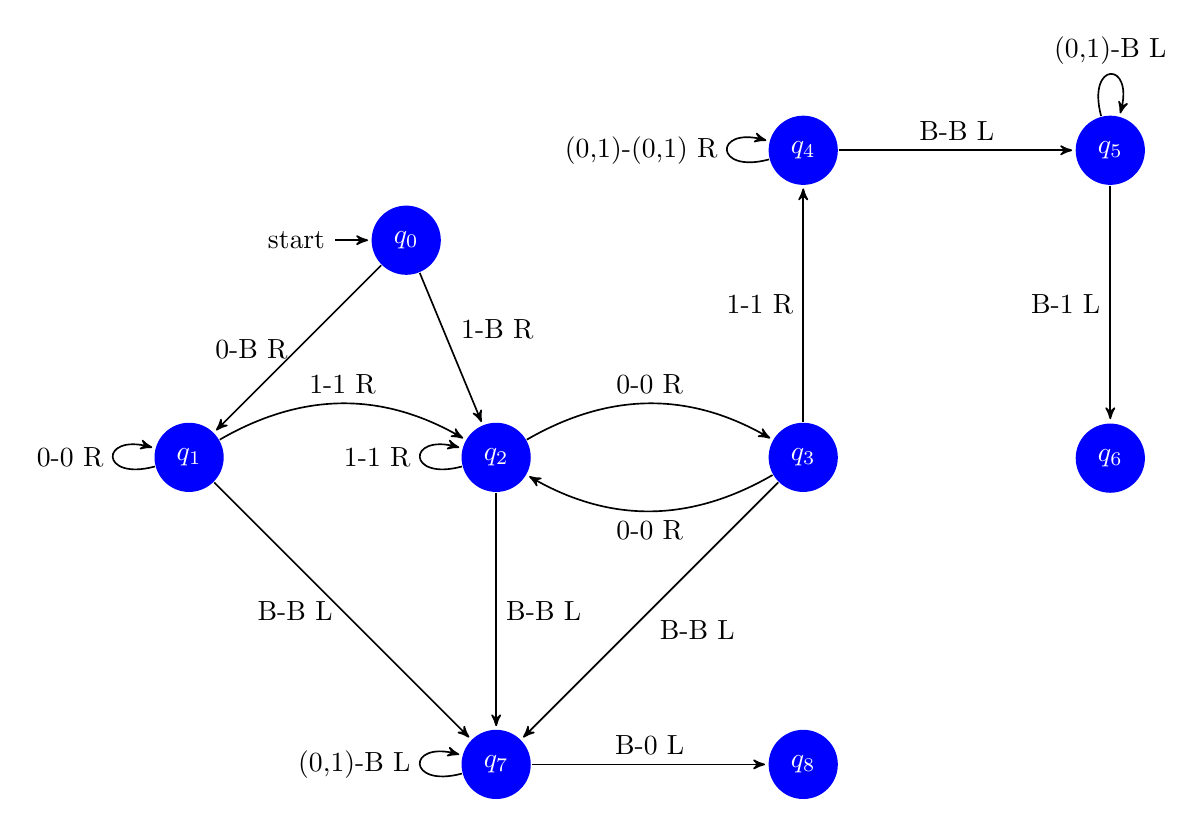
\begin{tikzpicture}[->,>=stealth',shorten >=1pt,auto,node distance=3cm,semithick]
  \tikzstyle{every state}=[fill=blue,draw=none,text=white]
	\node[state, initial] (q_0) {$q_0$};
	\node[state, below left=of q_0] (q_1) {$q_1$};
	\node[state, right=of q_1] (q_2){$q_2$};
	\node[state, right=of q_2] (q_3) {$q_3$};
	\node[state, below=of q_2] (q_7) {$q_7$};
	\node[state, right=of q_7] (q_8) {$q_8$};
	\node[state, above=of q_3] (q_4) {$q_4$};
	\node[state, right=of q_4] (q_5) {$q_5$};
	\node[state, accepting, below=of q_5] (q_6) {$q_6$};
	
	\path[->]	
	(q_5) edge[left] node{B-1 L} (q_6)
	(q_5) edge[loop above] node{(0,1)-B L} (q_5)
	(q_4) edge[loop left] node{(0,1)-(0,1) R} (q_4)
	(q_4) edge node{B-B L} (q_5)
	(q_0) edge[left] node{0-B R} (q_1)
	(q_0) edge node{1-B R} (q_2)
	(q_1) edge[left] node{B-B L} (q_7)
	(q_1) edge[loop left] node{0-0 R} (q_1)
	(q_1) edge[bend left] node{1-1 R} (q_2)
	(q_2) edge node{B-B L} (q_7)
	(q_2) edge[bend left] node{0-0 R} (q_3)
	(q_2) edge[loop left] node{1-1 R} (q_1)
	(q_3) edge node{B-B L} (q_7)
	(q_3) edge[bend left] node{0-0 R} (q_2)
	(q_3) edge node{1-1 R} (q_4)
	(q_7) edge node{B-0 L} (q_8)
	(q_7) edge[loop left] node{(0,1)-B L} (q_7);
\end{tikzpicture}

\newpage

A formal definition of the above Turing machine
\begin{wraptable}{r}{5.5cm}
	\centering
	\begin{tabular}{||c | c c c||} 
 		\hline
 		$\delta$ & 0 & 1 & B \\ [0.5ex] 
 		\hline\hline
 		$q_0$ & $q_1$ & $q_2$ & - \\ 
 		$q_1$ & $q_1$ & $q_2$ & $q_7$ \\
		$q_2$ & $q_3$ & $q_1$ & $q_7$ \\
 		$q_3$ & $q_2$ & $q_4$ & $q_7$ \\
 		$q_4$ & $q_4$ & $q_4$ & $q_5$ \\
 		$q_5$ & $q_5$ & $q_5$ & $q_6$ \\
 		$q_6$ & $Accepting$ & - &  $State$ \\
 		$q_7$ & $q_7$ & $q_7$ & $q_8$ \\
 		$q_8$ & $Rejecting$ & - & $State$ \\ [1ex] 
 		\hline
	\end{tabular}
\end{wraptable}

\begin{itemize}
	\item $Q \: = \: \{ q_0, \: q_1, \dots , q_8 \}$ 
	\item $\Sigma \: = \: \{0,\: 1 \}^*$ 
	\item $q_0$ is the start state
	\item $q_6$ is the "Accepting state"
	\item $q_8$ is the "Rejecting state" 
\end{itemize}
description: \\
$q_0$ marks the beginning of the tape with a $B$. $q_1, \: q_2 \: and \: q_3$ decide if there is a string $1v1$ string such that $v$ contains only $0's$ and $|v|$ is odd length. note, $q_1 \to q_2$ can only be achieved if a string starts with $0^n$ and eventually a $1$ is found, otherwise the string is rejected to $q_7$. When in $q_2$ a $1$ has been found and loops on $1$ until a $0$ is found. If there are odd number of $0's$ the head will be in $q_2$ and either a $1$ will be found $q_3 \to q_4$ and the string will be accepted and sent to $q_4$, or a $1$ will be found $q_2 \to q_2$ and the loop will start again, or a $B$ will be found in $q_1, \: q_2 \: or \: q_3$ and the string will be rejected to $q_7$. 
\\
\\
$(ii)$ Computation for above machine on string 01010: \\
$q_001010 \to 0q_11010 \to 01q_2010 \to 010q_310 \to 0101q_40 \to 01010q_4 \to$ \\
$0101q_50 \to 010q_51B \to 01q_50BB \to 01q_50BBB \to 0q_51BBBB \to q_50BBBBB \to$ 
$q_5BBBBBB \to q_61BBBBB$
\\ \\

\newpage

2. Turing machine for $f(x,y) = 2(x+y)$

\textbf{TM M \\}
\begin{tikzpicture}[->,>=stealth',shorten >=1pt,auto,node distance=3cm,semithick]
  \tikzstyle{every state}=[fill=blue,draw=none,text=white]
	\node[state, initial] (q_0) {$q_0$};
	\node[state, above=of q_0] (q_1) {$q_1$};
	\node[state, right=of q_0] (q_2){$q_2$};
	\node[state, right=of q_2] (q_3) {$q_3$};
	\node[state, below right=of q_6] (q_7) {$q_7$};
	\node[state, below=of q_2] (q_13) {$q_{13}$};
	\node[state, left=of q_7] (q_8) {$q_8$};
	\node[state, right=of q_3] (q_4) {$q_4$};
	\node[state, below=of q_3] (q_5) {$q_5$};
	\node[state, above=of q_3] (q_12) {$q_{12}$};
	\node[state, right=of q_5] (q_6) {$q_6$};
	\node[state, left=of q_8] (q_9) {$q_9$};
	\node[state, left=of q_9] (q_10) {$q_{10}$};
	\node[state, below=of q_10] (q_11) {$q_{11}$};
	
	\path[->]
	(q_0) edge node{1-0 R} (q_1)
	(q_0) edge node{B-0 R} (q_2)
	(q_13) edge[loop] node{1-1 L} (q_13)
	(q_13) edge node{0-0 R} (q_5)
	(q_9) edge node{0-0 R} (q_10)
	(q_10) edge node{B-1 L} (q_11)
	(q_11) edge[loop below] node{0-1 L} (q_11)
	(q_4) edge[loop] node{1-1 L} (q_4)
	(q_4) edge node{0-0 R} (q_5)
	(q_5) edge node{1-0 R} (q_6)
	(q_6) edge[loop] node{1-1 R} (q_6)
	(q_6) edge node{B-B R} (q_7)
	(q_7) edge[loop below] node{1-1 R} (q_7)
	(q_7) edge node{B-1 L} (q_8)
	(q_8) edge[loop below] node{1-1 L} (q_8)
	(q_8) edge node{B-B L} (q_9)
	(q_9) edge node{1-1 L} (q_13)
	(q_1) edge[loop] node{1-1 R} (q_1)
	(q_1) edge node{B-1 R} (q_2)
	(q_3) edge node{0-0 L} (q_12)
	(q_3) edge node{1-B L} (q_4)
	(q_2) edge[loop below] node{1-1 R} (q_2)
	(q_2) edge node{B-B L} (q_3);
\end{tikzpicture}

\newpage

A formal definition of the above Turing machine
\begin{wraptable}{r}{5.5cm}
	\centering
	\begin{tabular}{||c | c c c||} 
 		\hline
 		$\delta$ & 0 & 1 & B \\ [0.5ex] 
 		\hline\hline
 		$q_0$ & - & $q_1$ & $q_2$ \\ 
 		$q_1$ & - & $q_1$ & $q_2$ \\
		$q_2$ & - & $q_2$ & $q_3$ \\
 		$q_3$ & $q_{12}$ & $q_4$ & - \\
 		$q_4$ & $q_5$ & $q_4$ & - \\
 		$q_5$ & - & $q_6$ & - \\
 		$q_6$ & - & $q_6$ &  $q_7$ \\
 		$q_7$ & - & $q_7$ & $q_8$ \\
 		$q_8$ & - & $q_8$ & $q_9$ \\
 		$q_9$ & $q_{10}$ & $q_{13}$ & - \\
 		$q_{10}$ & - & - &  $q_{11}$ \\
 		$q_{11}$ & $q_{11}$ & - & - \\
 		$q_{12}$ & $Rejecting$ & - & $State$ \\
 		$q_{13}$ & $q_{5}$ & $q_{13}$ & - \\ [1ex] 
 		\hline
	\end{tabular}
\end{wraptable}

\begin{itemize}
	\item $Q \: = \: \{ q_0, \: q_1, \dots , q_13 \}$ 
	\item $\Sigma \: = \: \{0,\: 1 \}^*$ 
	\item $q_0$ is the start state
	\item $q_{11}$ is the "Accepting state"
	\item $q_{12}$ is the "Rejecting state" 
\end{itemize}
Description: \\
$q_0$ is the starting state and marks the beginning of the tape with a $0$. It also determines if $x=0$ (assuming $x=0,y=2$ will look like $\{ B11BB \dots \}$). If $x > 0$ then $q_1$ loops right until a $B$ is read. Once a $B$ is read it is changed to a $1$ and moves to $q_2$. However, if $x=0$ then $q_0$ changes the $B$ into a $0$ and moves straight to $q_2$. $q_2$ deals with $y$. If $y>0$ then $q_2$ loops on itself moving right on the tape until a $B$ is found. Otherwise, if $y=0$ the head moves left to $q_3$. If the head is looking at a $0$ this means that $x+y=0$ and the machine moves to $q_{12}$ and stops with the output $0$. When combining $x+y$ a $1$ is added where the $B$ separates $x \: and \: y$. $q_3 \to q_4$ removes the $1$ added, then $q_4 \to q_5$ moves the head back to the beginning of the tape and prepares for multiplication by two. 
The loop from $q_5 \to q_6 \to q_7 \to q_8 \to q_9 \to q_{13} \to q_5$ works in the following way; \\
When the loop is entered, the computation will look like so, $0q_511 \dots 1^n BB \dots$. $q_5$ will change the $1$ to a $0$ and move right till a blank is found. Once a blank is found, it will be left there to mark the center ($q_6 \to q_7$) and the machine will keep moving right over the $1's$ until another blank is found. for example: 
$011 \dots 1^n Bq_7BBB \dots \to 011 \dots 1^n q_8B1BB \dots$. $q_8$ will keep moving left over all the $1's$ until a blank is found (the marker for the center), then the machine continues to move left over all the $1's$ ($q_9 \to q_{13} \to q_5$) and the loop starts again. \\
If a $0$ is found in state $q_9$, this means that the multiplication loop is over, example: $000 \dots q_9 0^nB111 \dots 1^{n-1}$, $q_{10} \to q_{11}$ changes the $B$ (center marker) to a $1$ and finally $q_{11}$ loops left, changing all the $0's$ to $1's$.

\newpage

3.(a)$A\&B$ are infinite in size. Also, $N\approx A$ and $N\approx B$ where $N$ is the set of natural numbers.\\ \\

(i) $A \cup B$ is countably infinite: yes\\
We know that $A\&B$ are both countably infinite. Let $A=\{a_0, a_1, \dots, a_i \dots \}$ and $B=\{b_0, b_1, \dots, b_i \dots \}$ using the following function:
\[ f(n) = 
	\begin{cases}
	b_{n/2}				& \quad \text{if } n \text{ is even} \\
	a_{\frac{n+1}{2}}	& \quad \text{if } n \text{ is odd}
	\end{cases}
\]  We can now see that $f(n)$ has a bijection on the natural numbers. This means that $A \cup B$ also has a bijection on the natural numbers and by the definition of "countably infinite" $A \cup B$ remains countably infinite.   \\ \\

(ii) $A \cap B$ is countably infinite: yes\\
Since we know A \& B are countably infinite we know $A \cap B \subseteq A$ and A is countably infinite. To be more specific, Let $A=\{a_0, a_1, \dots, a_i \dots \}$ and $B=\{b_0, b_1, \dots, b_i \dots \}$. We can create a bijection between $N \approx A \cap B$ such that $A \cap B = \{a_0 \cap b_0, a_1 \cap b_1, \dots, a_i \cap b_i \dots \}$. Hence, by the definition of "countably infinite" $A \cap B$ remains countably infinite.   \\ \\

(iii) $A - B$ is countably infinite, where $ \{ x | x \in A \: \& \: x \notin B \: \} $: depends \\
\begin{enumerate}
	\item If $A = B$ then $A-B = \emptyset$ which is finitely countable. 
	\item If $\{ \forall a \in A \: | \: a \notin B) \}$ then $A$ remains unchanged and is still countably infinite. 
	\item If $\{ \exists a \in A \: | \: a \in B \}$ then we know that $A - B \neq \emptyset$ but we don't know if it is still infinity large or finitely large. We do however still know that it is countable because we can still have a bijection to the natural numbers. Therefore, $A - B$ is either finitely countable or infinitely countable.
\end{enumerate} 

\newpage

3. (b) Let F be the set of all total unary functions $f: N \to N $ and $F_{TC}$ be the set of all total unary Turing-computable functions $f: N \to N$.\\
Let $f^1_i$ be the unary function from $N$ into $N$ computed by Turing machine $M_i$. Now, let $F^k_i$ be the k-ary function from $N^k$ into $N$ computed by machine $M_i$.
We can now see that for each $k \geq 1$ the set of $F_{TC} = \{ f^k_1, f^k_2, f^k_3, \dots \}$ which is a countably infinite set.  \\
We can also see that the set $F_{TC} \subseteq F$ which implies that $F$ is also countably infinite. If we took away the set $F_{TC}$ from the set $F$ ($F_{TC}-F$) then we would be left with the set of all total unary functions that are not Turing-computable. This is also a sub set of $F$ and therefore is also countably infinite.


\newpage
4. Does Godel's incompleteness theorem imply the impossibility of Hilbert's programme? \\
\\
Hilbert's program was designed to provide a secure foundation for all mathematics. This proposition included a requirement for all mathematical statements to be written in precise formal language and manipulated according to well defined rules (formal system). Completeness where a proof that all true mathematical statements can be proved in the adopted formal system. Consistency where a proof has no contradictions that can be obtained in the formal system. Decidability where an algorithm can be constructed for deciding, in the formal system, the truth or falsity of any mathematical statement. Finally, Conservation where a proof that any result about "real objects" obtained using "ideal objects" can be restated without using ideal objects. \\ \\
Godel's incompleteness theorem shows that there is a gap between "truth" and "proof" where there are some true statements which can not be proved within any mathematical system. Axioms are an important part of Godel's incompleteness theory. If we do not have all of the axioms to prove a true statement we can just add that as a new axiom and it will expand what we can prove within mathematics. This is very important for Godel because we are trying to prove that there will be a set of axioms from which we can deduce all truths of mathematics. Godel produced what is known as Godel coding. Godel devised a way to code all mathematical statements, including whether they are true or not. This gave him the ability to compare statements with one another and deduce a proof. \\

A simple example of the paradox that Godel's incompleteness theorem shows is this. Imagine the statement "This statement cannot be proven mathematically" this statement is obviously either true or false. So, lets start by assuming the statement is false. That would mean "This statement can be proven mathematically" is true, but a provable statement must be true, so we have started with something we assumed was false and now we have deduced that it is true. This is a contradiction. This is a problem for Hilbert's programme because consistency requires a proof to have no contradictions. This means our statement "This statement cannot be proven mathematically" can not be false, so it must be True. But now we have a statement "This statement cannot be proven mathematically" is true, but can not be proven. Therefore, we have found a true statement which can not be proven true within that system. This is another problem for Hilbert's programme because completeness states that a true statement can be proven.  \\

Godel's theorem goes on to explain that we could add the axiom to make the above truth statement provable in our system, but that will not help as no matter what, a new statement can always be shown true but not provable in our new system. As I understand it, no matter how much you expand mathematics by adding axioms, the system will always be missing something. This would make it impossible to create a formal system of mathematics and again adding to the impossibility of Hilbert's programme. \\

In conclusion, Godel's incompleteness theorem does imply the impossibility of Hilbert's programme ever being satisfied.



\end{document}